\chapter{Methods}
\label{sec:methods}

Our overall goal is to extract Ly$\alpha$ observables from cosmological zoom-in simulations of massive galaxies in evolution in post-processing.
To do this, we construct a pipeline in which we smooth the particle data from snapshots onto an octree (a particular kind of grid with adaptive resolution) on which we perform ionizing radiative transfer, to determine the ionization state of the gas in the halo.
Then we use Ly$\alpha$ Monte-Carlo radiative transfer (MCRT) in order to compute the escape fraction from the simulation domain, as well as surface brightness images, moment maps, and spectra of the Ly$\alpha$ line.
In what follows, we go into substantially more detail about each of these numerical techniques.

\section{Cosmological Hydrodynamic Zoom Galaxy Formation Simulations}

The galaxy formation simulations studied here are a part of the MassiveFIRE suite of cosmological zoom-in hydrodynamic galaxy formation simulations \citep{Feldmann2016, Feldmann2017}, which itself is a part of the Feedback in Realistic Environments (FIRE) project.
In particular, these simulations employ the FIRE-2 suite of physics.
These physics modules are fully described in \citet{Hopkins2018}, and we point the reader to this work, summarizing the salient details.

The initial conditions for the MassiveFIRE simulations are generated with the {\sc music} initial conditions generator for a $(100/h \ {\rm Mpc})^3$ box.
We first run an initial low-resolution simulation, from which we selected particular halos for re-simulation at much higher resolution.
For these halos, the region encompassing the high-resolution particles was selected with a convex hull filter selecting all particles within $3$ virial radii of the halo at $z=2.$
These particles were then split to obtain higher mass resolution, and the entire simulation was re-run with a final mass resolution of the high-resolution particles of $m_{\rm DM} = 1.7 \times 10^5 M_\odot$ and $m_{\rm baryon} = 3.3 \times 10^4 M_\odot$ for dark matter and baryons, respectively.

The simulations themselves are run with {\sc gizmo} \citep{Hopkins2015} with the hydrodynamics run in Meshless Finite Mass (MFM) mode.
The FIRE-2 simulations use a metallicity-dependent treatment of radiative heating and cooling that covers a temperature range from 10 to $10^{10}$ K, and includes free-free, photoionization, recombination, Compton, photoelectric and dust collisional, cosmic ray, molecular, metal-line, and fine-structure processes.
They also include cooling and abundances of 11 elements, and include sub-grid diffusion of metals via turbulence.
These simulations include star formation in dense and self-gravitating gas \citep{Hopkins2013}, and stellar feedback channels that include radiation pressure, photoionization, photoelectric heating, O-star and Asymptotic Giant Branch (AGB) driven stellar winds, and Type I and II Supernovae.
Supermassive black holes are included in the simulations, but followed passively, meaning that feedback from an active galactic nuclei (AGN) is not included.
This said, black holes accreted following the torque-limited accretion model of \citet{Anglesalcazar2017a,Anglesalcazar2017b}.
In this paper, we examine $4$ massive halos, whose physical properties are described at $z=2$ and $z=5$ in Tables~\ref{table:sims2} and ~\ref{table:sims5} respectively.
We use a $150 \times 150$ kpc box to encompass $2$ virial radii about the central galaxy at $z=2$, which we identify with a friends-of-friends search using star particles.
These halos have the same initial conditions as those monikered ``A1", ``A2", ``A4", and ``A8" from \citet{Feldmann2016}.

\begin{table*}
\caption{Properties for our 3 model halos at $z=5$, within our $150 \times 150\ \rm kpc$ box}
\centering
\begin{tabular}{l r r r r}
Name & $M_{\rm DM}$ & $R_{\rm vir}$ & $M_{\rm star}$ & SFR \\
   & ($M_\odot$) & (kpc) & ($M_\odot$) & ($M_\odot / \rm yr ^{-1}$)\\ \hline
A1 & $9.72\times 10^{11}$ & $5.60 \times 10^1$  & $2.07 \times 10^{10}$ & $3.11\times10^1$ \\ \hline
A2 & $3.98\times 10^{11}$ & $4.20 \times 10^1$  & $3.81 \times 10^{9}$ & $2.65\times10^1$ \\ \hline
A4 & $2.98\times 10^{11}$ & $3.81 \times 10^1$  & $1.32 \times 10^{9}$ & $4.70\times10^0$ \\ \hline
A8 & $3.04\times 10^{11}$ & $3.84 \times 10^1$ & $9.38 \times 10^{8}$ & $8.18\times10^0$ \\
\hline
\end{tabular}
\label{table:sims2}
\end{table*}

\begin{table*}
\caption{Properties for our 3 model halos at $z=2$, within our $150 \times 150\ \rm kpc$ box}
\centering
\begin{tabular}{l r r r r}
Name & $M_{\rm DM}$ & $R_{\rm vir}$ & $M_{\rm star}$ & SFR \\
   & ($M_\odot$) & (kpc) & ($M_\odot$) & ($M_\odot / \rm yr ^{-1}$)\\ \hline
A1 & $1.64\times 10^{12}$ & $1.20 \times 10^2$  & $1.78 \times 10^{11}$ & $6.55\times10^1$ \\ \hline
A2 & $2.00\times 10^{12}$ & $1.29 \times 10^2$  & $2.98 \times 10^{11}$ & $1.68\times10^2$ \\ \hline
A4 & $1.63\times 10^{12}$ & $1.19 \times 10^2$  & $1.41 \times 10^{11}$ & $7.15\times10^1$ \\ \hline
A8 & $1.92\times 10^{12}$ & $1.26 \times 10^2$ & $8.06 \times 10 ^{10}$ & $8.79\times10^1$ \\
\hline
\end{tabular}
\label{table:sims5}
\end{table*}

\begin{figure}
   \centering
   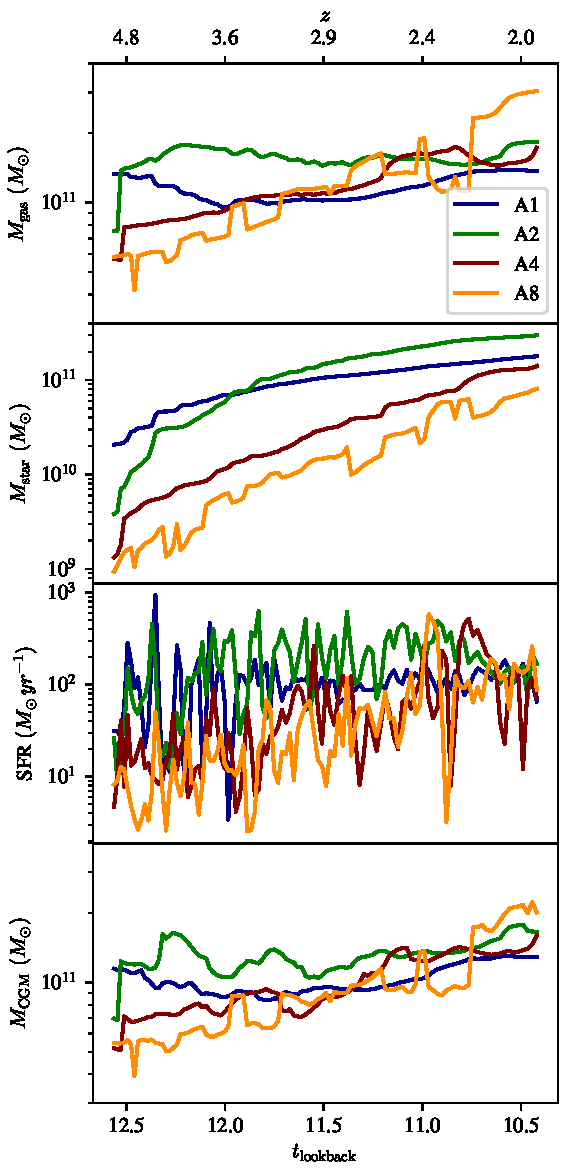
\includegraphics[width=\textwidth,height=0.85\textheight,keepaspectratio]{figures/properties_redshift.pdf}
   \caption{Evolution of physical properties of each halo.
   We show (from top to bottom) the total gas mass, stellar mass, star formation rate, and circumgalactic medium gas (defined as all gas in the box not associated with the central galaxy).
   The physical properties are computed over the $150 \times 150\ \rm kpc$ box employed for our radiative transfer calculations.}
   \label{fig:properties_redshift}
\end{figure}

\section{Computing the Ionization State of the Gas}
\label{sec:lycrt}

Our end goal is to simulate Ly$\alpha$ emission and radiative transfer in these simulations.
Since we want to do this from first principles as much as is reasonably possible, we first present the rate equations we will use for emission due to recombinations and collisions.

\begin{equation}
\label{eq:j_rec}
    L_{\rm Ly \alpha}^{\rm rec} = h\nu_{\alpha} \int P_B(T)\,\alpha_B(T)\,n_e\,n_{\HII}\,\mathrm{d}V
\end{equation}

\noindent where $h$ is Planck's constant, $\nu_{\alpha}$ is the rest-frame frequency of Lyman-$\alpha$, $P_B(T)$ is the Ly$\alpha$ conversion probability per recombination event and $\alpha_B(T)$ is the case-B recombination coefficient \citep{Cantalupo2005, Dijkstra2014, Hui1997}, $T$ is the temperature of the gas, $n_{e}$ is the electron number density, and $n_{\HII}$ is the ionized hydrogen number density.

For emission due to collisions, the Ly$\alpha$ luminosity is,
\begin{equation}
\label{eq:j_col}
    L_{\rm Ly \alpha}^{\rm col} = h\nu_{\alpha} \int C_{1s2p}(T)\,n_e\,n_\HI\,\mathrm{d}V
\end{equation}

\noindent where $C_{1s2p}(T)$ is the temperature-dependent collisional rate coefficient \citep{Scholz1991}, and $n_{\HI}$ is the number density of neutral hydrogen.

From these equations, we can see that there are two quantities that we need to know accurately: The gas temperature and ionization state.
The simulations we have snapshots from do contain mechanisms to calculate both of these, but in both cases there are reasons to doubt the on-the-fly calculations.
This is not to say that the on-the-fly calculations have been done carelessly; these systems are extremely complex and since the ionization state, temperature, and UV field all depend on each other and accurate calculation of any of those properties requires an iterative solver.
Such an iterative solver requires more compute time than is easy to justify doing at every time step in a large-scale simulation; but we can do this in post-processing for just the time steps at which we have snapshots without massive computational expense.

Therefore, our first step in post-processing is to compute a more accurate ionization state of the gas, by doing ionizing UV radiative transfer.
All the radiative transfer in this work is done on an octree, even though the snapshot data is all from SPH simulations.
We use an octree because the implementation is much simpler, and most likely much faster than attempting radiative transfer on an SPH field; in an octree we can track which cell a Monte Carlo is within and simply look up the gas properties in the tree.
When we deposit the SPH data onto the octree we can impose refinement or stopping criteria; in our case we can set a maximum number of particles in a cell and a minimum cell size.
Unless otherwise specified, in this work we set the maximum number of particles to 1 (that is, keep refining until there is only one particle per octree cell) and the minimum cell size to $0.01\ \rm{kpc}$.

In some sense, this conversion from SPH particles to an octree is necessarily lossy, since we cannot convert from an octree structure back to the SPH representation.
Remember that the point of this different data structure is to have a different representation of the represented gas density field (and other properties), not to do efficient neighbor-searches which is a common application of octrees.
Therefore, we must concede that there is something lost in this deposition onto an octree.
But we can minimize this change, in fact arbitrarily so.
SPH particles are not points; they do not exist at only one location in space and instead define a density field, and since we can evaluate this density field at any location in space there is no particular reason to stop refining an octree at the limit of one particle center per cell.
We \emph{could} sub-divide the space more, in a process often called over-refining and thus eventually reach at every point in space an octree cell size such that the discontinuities introduced by the discretized structure do not exceed the imprecisions in the original SPH data.

\iffalse
\begin{figure}[H]
    \centering
    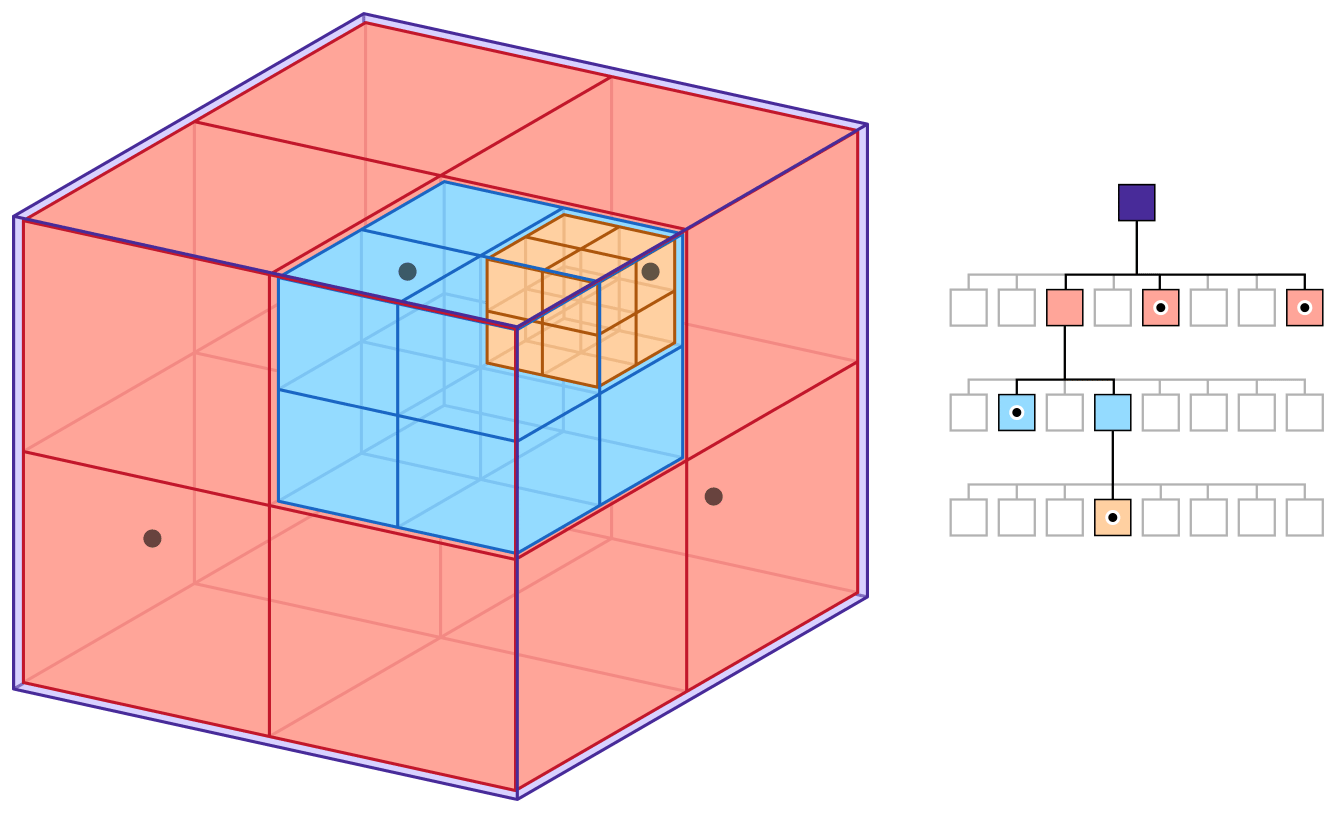
\includegraphics[width=\textwidth,keepaspectratio]{figures/apple_octree.png}
    \label{fig:octree_refinement}
    \caption {
        A diagram of the octree refinement process, in a scenario where we require that an octree cell not contain more than one particle.
        On the left is a spatial representation of the tree, on the right we represent the tree in the more traditional diagram for trees.
        Image from https://developer.apple.com/documentation/gameplaykit/gkoctree
    }
\end{figure}
\fi

\begin{figure}[H]
   \centering
    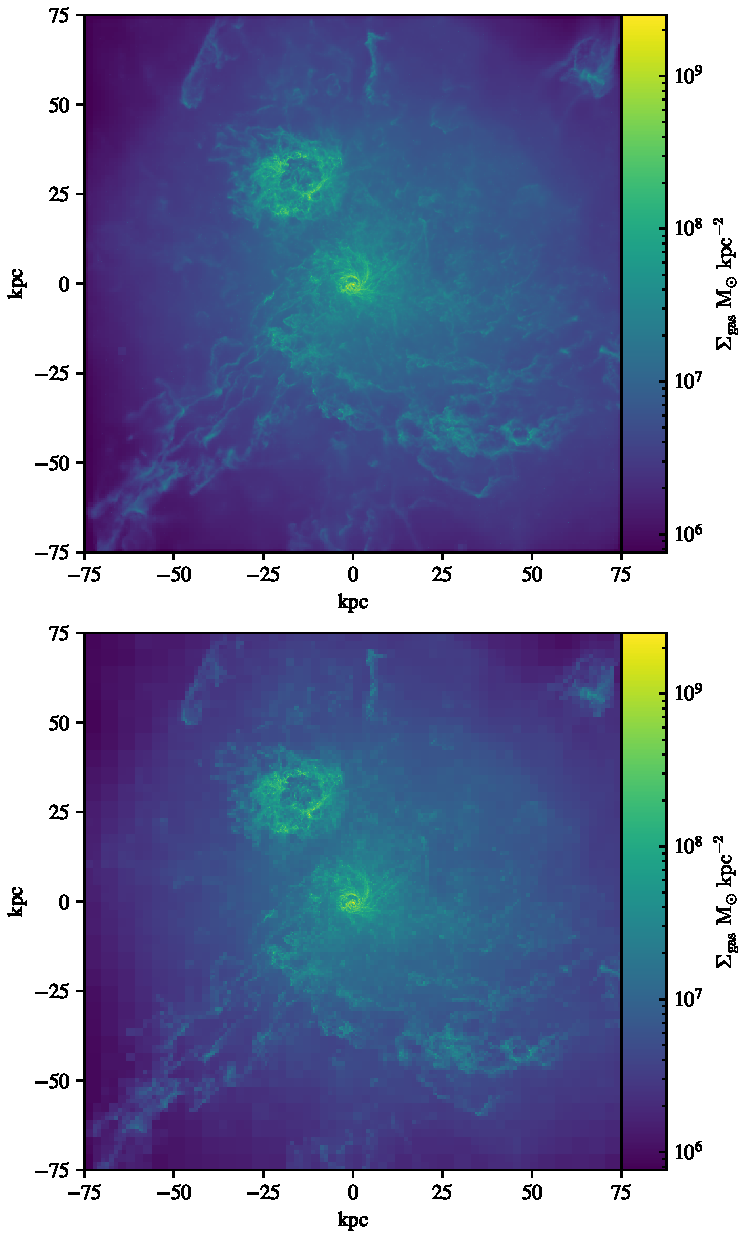
\includegraphics[width=\textwidth,height=0.85\textheight,keepaspectratio]{figures/octree_resolution.pdf}
    \caption{
        Top: A gas density projection of the $z = 2.0$ snapshot from MassiveFIRE halo A4, after being deposited onto an octree with the default settings we use in this work: Minimum cell size $0.01\ \rm{kpc}$, and no limit on the number of particles per cell.
        Bottom: The same snapshot but deposited where we require 64 particles per cell. Here, the octree cells are much more visible, and one can see that the octree cell size traces the gas density, which is the objective of such particle or adaptive grid schemes. We want better resolution where the gas density is greater.
    }
   \label{fig:octree_resolution}
\end{figure}

The deposition of the SPH data and subsequent calculation of the ionization state is done by {\sc lycrt} (Lyman-Continuum Radiative Transfer) \citep{Ma2015}.
{\sc lycrt} is a Monte-Carlo radiative transfer code that iteratively computes the gas ionization state by emitting rays from both stars and a uniform UV background.
These rays are subject to scattering by HI along with dust scattering and absorption, using the dust opacity formulation from \citet{Li2001}, and the passage of these rays through octree cells is used to compute the ionizing UV field.
We assume a redshift-dependent UV background with intensity as described in \citet{Faucher-Giguere2009}.

Here we describe a general overview of {\sc lycrt}, which is an ionizing radiative transfer code.
Most of this procedure also applies to {\sc COLT}, the codebase we use to do the Ly$\alpha$ radiative transfer though the details are somewhat different.

We start by selecting a location to emit a photon from.
This, like many other steps, must be done randomly but on a particular probability distribution.
In this case we need to select a star particle to emit from based on the distribution of luminosities of all the star particles.

From an SPH simulation we only know that there are star particles with a position, velocity, mass, and age.
These star particles do not represent individual stars, in the simulations we use here they range from $1.5\times10^{4}\ \rm{M}_{\odot}$ to $5.1\times10^{6}\ \rm{M}_{\odot}$.
Since these star particles represent something more like clusters of stars (due to the limited resolution we need to make this whole field computationally feasible) we use stellar population synthesis to treat each star particle as an entire stellar population.
In this project we use Binary Population and Spectral Synthesis ({\sc bpass}) spectral libraries (notable because they include the effect of binary stars \citep{Eldridge2008}) to find the brightness of each star particle at all energies greater than the ionization energy of hydrogen.
Now, given the (ionizing) brightness of all the stars it's possible to randomly sample them.

PRNG (pseudo-random number generator) implementations produce numbers on the interval $[0, 1)$; so we construct a cumulative distribution for the star particles in the simulation (which covers the same interval), then do a binary search inside our CDF array for a random number to select the index of the star that emits this photon.
Now we have a position for the photon, we still need a direction and initial energy (or frequency, or wavelength).
The direction is randomly generated over the unit sphere, but the initial energy is a bit more interesting.
In the {\sc lycrt} codebase this is drawn from a power law distribution between the ionization energy of hydrogen and the first ionization energy of helium.
This is a quite good approximation for stars, but since we will much later use this same process simulate AGN in \S~\ref{sec:agn}, it might be beneficial to control this distribution based on the luminosity of the emitting particle.

Now that we've created an MCRT photon packet it moves through the simulation in discrete jumps from scattering to scattering.
We start by computing the opacity $\kappa$ in the octree cell that the photon currently resides in, from the following equation:
\begin{equation}
    \label{eq:lycrt_opacity}
    \kappa = 6.0^{-18} E^{3} \rho n_{\rm{HI}} + \kappa_{\rm{dust}}
\end{equation}

where $E$ is the energy of the photon, $\rho$ is the density of the gas, $n_{\rm{HI}}$ is the number density of neutral hydrogen, $\kappa_{\rm{dust}}$ is energy-dependent dust opacity from \citet{Weingartner2001}.
We then draw a random optical depth which the photon shall traverse until it scatters, and use the known opacity of the cell to convert that optical depth to a distance.
If traveling this distance along the photon's current direction would place the photon outside of the current grid cell, we find the cell it will cross into and repeat the conversion to distance based on the remaining optical depth.
Once we have exhausted the randomly chosen optical depth, another random number is drawn to determine if the photon is scattered or absorbed by dust.
When photons are scattered, we re-draw a random direction, and modify its energy to be just above the hydrogen ionization energy.
This process ends when a photon escapes from the simulation or is absorbed by dust.

Photons are also emitted uniformly from the UV background, and propagate inwards toward the simulation domain.
These photons are mostly the same, except their initial energy distribution is drawn from a uniform distribution between the ionization energy of hydrogen and the first ionization energy of helium, instead of a power law distribution.

As a photon passes through grid cells, it adds to the UV field in that cell according to its energy and the distance through that cell it traversed.
Therefore, by simulating many of these MCRT photon packets we are able to estimate the UV field in all the cells in the simulation and use this UV field along with the temperature in each cell to recompute the ionization state for every cell \citep{Kasen2006}.

It is worth nothing that this ionization solver does not update the gas temperature based on the UV field.
While the investment to add this effect is not huge, it is very unlikely to have a large impact because it would mostly alter the temperature of highly ionized regions of the simulation, wherein the Ly$\alpha$ luminosity is not particularly sensitive to temperature.
In addition to this though, it is worth noting that even though this ionization state solving system is not self-consistent, adding the effect on temperature does not make it self-consistent because the underlying hydro simulation all this work is based on already contains an approximate prescription for these effects.
At some point we need to admit that this work is all approximate and stop adding physics to the model somewhere, and here is where we draw the line in post-processing (thought it would be nice if there were accurate on-the-fly ionization and temperatures due to radiative transfer).


\section{Ly\texorpdfstring{$\alpha$}{a} Emission and Radiative Transfer}
\label{sec:colt}

The Ly$\alpha$ Monte Carlo radiative transfer calculations are performed using the Cosmic Ly$\alpha$ transfer Code \textsc{colt} \citep{Smith2015}.
In this dissertation we only provide a brief overview of the most important details in Ly$\alpha$ radiative transfer.
This project was focused around using and extending an existing codebase, and therefore there are elements of a high-quality Ly$\alpha$ MCRT codebase such as \textsc{colt} that this project relies upon but did not interact directly with.

\textsc{colt} models the  emission of Ly$\alpha$ photons due to hydrogen recombination and radiative de-excitation of collisionally excited hydrogen, and accounts for scattering due to neutral hydrogen, and scattering and absorption due to dust.
To do this, \textsc{colt} generates Monte Carlo photon packets in octree cells with probability proportional to the Ly$\alpha$ luminosity of each cell.
This luminosity is based on hydrogen emission due to recombination and radiative de-excitation of collisionally excited hydrogen, which we presented previously in Eq. \ref{eq:j_rec} and Eq. \ref{eq:j_col}.

The Ly$\alpha$ radiative transfer in {\sc colt} proceeds for the most part like that described above for {\sc lycrt}, but with some important differences.
When doing ionizing radiative transfer, we can ignore a number of effects because we are modeling continuum behavior and the precise frequency of photon packet being simulated does not have a large impact on its propagation through the simulation.
In Ly$\alpha$ radiative transfer we do not have this luxury because the opacity of neutral hydrogen is sensitive to the frequency of the incident photon.

Specifically, the local Ly$\alpha$ absorption coefficient is given by
\begin{equation}
   \label{eq:kalpaha}
   k = n_{\rm H _I} \sigma(\nu),
\end{equation}
where $\sigma_\alpha(\nu)$ is the Ly$\alpha$ cross-section, which at line center is $5.898\times 10 ^{-14}\ T ^4\,\rm cm^2$.
This cross section is importantly a strong function of the photon's frequency and is given by
\begin{equation}
    \sigma(\nu) = f_{12}\frac{\sqrt{\pi} e^{2}}{m_{e} c \Delta\nu_{\rm{D}}} H(a, x)
\end{equation}
where $f_{12} = 0.4162$ is the oscillator strength of the Ly$\alpha$ transition, $\Delta\nu_{\rm{D}}$ is the thermal Doppler width of Ly$\alpha$ given by $(v_{\rm{th}}/c)\nu_{0}$, and $H(a, x)$ is the Hjerting-Voigt function which describes the line profile.
This line profile depends on the damping parameter which is a straightforward function of temperature:
\begin{equation}
    a \equiv \frac{\Delta \nu_{\rm{L}}}{2\Delta \nu_{\rm{D}}} = 4.702 \times 10^{-6} T
\end{equation}
and the frequency of the photon, but in this area it is typical to express frequency as a dimensionless number of Doppler widths from line center,
\begin{equation}
    x \equiv \frac{\nu - \nu_{0}}{\Delta\nu_{\rm{D}}}
\end{equation}

The exact formulation of this $H(a, x)$ is the convolution of a Lorentzian and Maxwellian distribution and is therefore highly impractical to be evaluating constantly to do our optical depth calculations.
Therefore, there is some history of approximations for this function which all use some criteria to split the distribution into a core and a wing component, and apply different approximations in each regime.
In this work we use a continued fraction expansion centered around $0$, $\infty$, and on the interval $3 < x^{2} < 25$.
This provides better than $1\%$ error in the value of $H(a, x)$ across the range of frequencies and temperatures that we encounter in the simulations, while being efficient enough that it is not a major contributor to the runtime of MCRT simulations.

Scattering events in Ly$\alpha$ radiative transfer are also much more complex than in a continuum radiative transfer code.
Whereas before we described a scattering event as simply changing the direction of the photon packet, when frequency is very important we need to consider other effects.
A Ly$\alpha$ scattering event is not instantaneous; there is a rapid absorption and re-emission by the interacting atom and therefore we need to properly account for the atom's initial velocity and the recoil effect.
Therefore, given an atom with initial velocity $\vec{u}_{\rm{atom}}$ and a photon packet with initial direction $k_{i}$ and initial frequency $x_{i}$, we can compute the final direction $k_{f}$ and frequency $x_{f}$:
\begin{equation}
    x_{f} = x_{i} + (\vec{k}_{f} - \vec{k}_{i})\cdot \vec{u}_{\rm{atom}} + g(\vec{k}_{i}\cdot\vec{k}_{f} - 1)
\end{equation}
where $g$ is the recoil parameter defined as
\begin{equation}
    g \equiv \frac{h\Delta\nu_{\rm{D}}}{2k_{B}T} = 2.536 \times 10^{-6}T \approx 0.54 a
\end{equation}
Drawing a random velocity for the scattering atom is one of the most significant computational challenges in Ly$\alpha$ MCRT.
The perpendicular component is drawn from a simple Gaussian distribution, but the parallel component is affected by the presence of the resonant line.
Therefore, the distribution of the parallel component $u_{\parallel}$ is given by
\begin{equation}
    f(u_{\parallel}) = \frac{a}{\pi H(a, x)}\frac{e^{-u_{\parallel}^{2}}}{a^{2} + (x - u_{\parallel})^{2}}
\end{equation}

In general, to convert outputs from a pRNG which produces values on the interval $[0, 1)$ to an arbitrary distribution, we treat the values from the pRNG as values of the CDF of the desired distribution.
So to convert from a pRNG to some arbitrary distribution, we require that the desired distribution have a density function that we can integrate, then invert.
This possible for \emph{some} distributions, but for distribution of parallel atom velocities it is particularly challenging, in a numerical and computational sense and beyond the scope of this work.
We defer the reader to \citep{Smith2015} for a full description of the methodology used for this in \textsc{COLT}.

\subsection{Core-Skipping}
\textsc{colt} includes a few other acceleration schemes other than the approximation for $H(a, x)$, the most important of these is core-skipping which we mention here briefly.
Core-skipping is an approximation wherein photon packets which scatter near the line center in a region of the simulation with high opacity are promoted to the wings of the line, where they will see much less opacity on their next scattering.
This is done by randomly generating scattering atom velocities until one is chosen that would shift the photon packet's frequency sufficiently far away from the line center.
The formulation of this optimization currently present in \textsc{colt} is worth 10x in runtime, and produces an error no greater than a $3\%$ in the escape fraction of the simulation.

\subsection{Dust Absorption}
Following \citet{Laursen2009}, we assume SMC-like dust properties with an effective cross-section per hydrogen atom of $3.95\times10^{-22}\ \rm{cm}^{2}$, and fiducial albedo of 0.32.
The SMC may not be a particularly good model for the much older galaxies that this work studies, but it is the most similar in metallicity of the galaxies for which we have good dust parameters.
In contrast with previous works such as \citet{Laursen2007} and previous uses of \textsc{COLT} such as \citet{Smith2015}, we now treat dust absorption as a continuous process, such that each photon packet has a weight that is attenuated according to the traversed dust optical depth.

In a naive implementation of continuous dust absorption, every photon must eventually escape the simulation domain.
This increases the runtime of an MCRT simulation massively ($>100$x) so we introduce a threshold at which we discard photon packets from the simulation.
If one is investigating bulk properties of a system such as escape fraction it is easy to choose a threshold based on what fraction of total luminosity could be discarded from the simulation and not represent a dominant source of error.
In this work we are also interested in studying surface brightness images which span a few orders of magnitude and so we have chosen a much more conservative value for this discard threshold of $e^{32}$.

This change to the dust absorption mechanism also offers an opportunity to do some interesting additional work.
Specifically, it opens up the possibility to study which octree cells in the simulation domain absorb energy from photons, or alternatively in which cells a photon is substantially absorbed.
In the usual scheme wherein we draw a random number at each scattering to determine if the photon is absorbed, for our usual number of photons $(10^{7})$ is within a factor of 2 of the typical number of octree cells in a $z=2$ snapshot.
Therefore, in the normal scheme if we are to simply record cells that absorb a photon, we have rather poor statistics over most of the simulation.
But with a continuous absorption domain we could record in each cell how much energy it absorbs due to dust from the Ly$\alpha$ that passes through it, without significantly increasing the memory consumption of the simulation.
The amount of memory required to store each photon's entire path through the simulation would be massive, but if we wanted to answer questions like ``Which cells were most important to the absorption of this photon packet'' one could use a streaming algorithm like heavy hitters to record only the few most impactful cells on every photon packet.

\subsection{Luminosity Boosting}
Recall that in these simulations, to emit a Ly$\alpha$ photon packet we draw from the cumulative distribution of octree cell luminosities.
This need not necessarily be the case, for photon packets.
It must be the case for the Ly$\alpha$ energy budget, but luminosity boosting is a mechanism that can let us decouple the Monte-Carlo sampling from the luminosity distribution in a simulation.
And most importantly, we are interested in manipulating the sampling strategy because it is a way to control and hopefully improve the convergence of some aspect of these simulations.

The particular scheme we have introduced uses an input parameter $j_{\rm exp}$ such that the probability of a cell $i$ emitting a photon packet is:
\begin{equation}
    P_{i} = L_{\rm Ly \alpha, i} ^{j_{\rm exp}}
\end{equation}
That is, $j_{\rm exp} = 1.0$ is equivalent to no boosting, and $j_{\rm exp} = 0.0$ means that the emission from every cell is sampled equally.
There is no principled reason to restrict $0 <= j_{\rm exp} <= 1.0$, and depending on the exact escape properties values outside that range may be useful.

This implementation of luminosity boosting allows us to emit more photons of lower initial weight from low-luminosity regions, thus with luminosity boosting we can converge the contribution of low-emissivity areas faster.
Without luminosity boosting we converge the effects of octree cells proportionally to their luminosity, which is approximately optimal for converging the bulk properties fastest.

The value of $j_{\rm exp}$ can (should) be tuned to accelerate convergence at a particular surface brightness level.
For most of our simulations, we need good convergence at least to a surface brightness of $10^{-18}\ \rm{erg}\rm{s}^{-1}\rm{cm}^{-2}\rm{arcsec}^{-2}$ because that is a typical sensitivity of Ly$\alpha$ surveys.
Simulating $10^7$ MCRT photon packets gets us close to this number, so to study this we compare a grid of $j_{\rm exp}$ values at $10^7$ photon packets to a single run at $10^9$ photon packets which we assume is converged everywhere.
We present this grid in Figure~\ref{fig:j_exp_profiles}.
From this figure we can see that $j_{\rm exp} \sim 0.8$ provides the best convergence.

\begin{figure}[H]
   \centering
   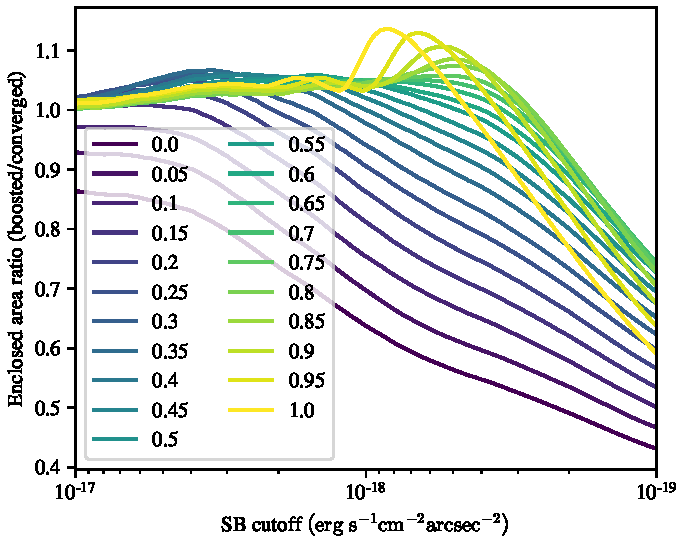
\includegraphics[width=0.9\columnwidth]{figures/profiles.pdf}
    \caption{
        Our usual simulations are run with $10^{7}$ photon packets.
        To produce this figure, we first run a simulation with $10^{9}$ photon packets, from which we take a surface brightness image and use this as if it's fully converged.
        Then, we run 21 simulations with different values of $j_{\rm exp}$ from $0.0$ to $1.0$ and compute the area of the surface brightness image enclosed by isophotes as a function of the isophotal level.
        In this figure, a fully converged simulation would be a horizontal line at $1.0$.
        Following a contour from the left to the right traces the convergence of the simulation at fainter and fainter regions of the image.
    }
   \label{fig:j_exp_profiles}
\end{figure}

However, this is just one possible formulation of luminosity boosting.
In particular, it's one of the simplest.
The general technique is to adjust both the probability of sampling emission from a cell and the weight that the sample is given.
That is, there is some function that maps octree cells (or position in space) to a probability of being sampled.
The weight $w$ is trivially determined from the weight function $W$ for any cell $i$ by the equation
\begin{equation}
    W_{i} = W(i)L_{i} / L_{\rm tot}
\end{equation}
In the weighting scheme we have so far discussed, the weight function depends on the luminosity of a cell, but that need not be the case.

Before, we mentioned that converging the effects of each cell proportionally to their luminosity is \emph{approximately} optimal for converging bulk properties.
The precisely optimal scheme would sample each cell with respect to its contribution to the overall luminosity.
The naive non-boosted is just close because for the MCRT work we are doing, the variation in cell luminosity is much greater than the variation in escape fraction from cell to cell.
So optimally, we would know for each cell in the simulation, what the escape fraction is for photons that originate in that cell.
We can determine this per-cell escape fraction from a \textsc{colt} run because we save the index of the cell a photon packet was emitted from, along with its emitted and escaping weight and therefore can compute for each cell $i$ for every photon $P$ with weight $W$ that originates from it,
\begin{equation}
    W_{i} = \frac{L_{i}}{L_{\rm tot}}f_{\rm esc}^{i} =\frac{L_{i}}{L_{\rm tot}} \sum_{p}\frac{W_{\rm escaping}}{W_{\rm emitted}}
\end{equation}
In practice, computing an accurate escape fraction to enable this optimal weighting scheme is limited by the unfortunate reality that accurately computing these weights is equivalent to computing converged bulk properties of the simulation.\\

\subsection{MPI and Work Scheduling}
Normally in such a codebase, one would distribute work to MPI ranks in large batches under the logic that communication overhead is rather large compared to the smallest possible unit of work (in our case an MCRT photon packet).
\textsc{colt} was originally designed this way, and indeed this scheme does incur minimal communication overhead.
The possibly-hidden cost is that there is a tradeoff between communication scheduling efficiency.
If we have $P$ photon packets to run, and $M$ MPI ranks, giving each rank $P/M$ photon packets results in a large variation in when each rank finishes its work and becomes idle.
With this naive scheme, we find that the allocated CPUs are only occupied for $\sim 70\%$ of the simulation's runtime.
A next logical step is to distribute work in batches of $P/(N\times M)$ for some tunable constant $N$, which would balance the per-message communication overhead with the variation in runtime for any batch of photon packets.
However, we could simplify this whole system by sending photon packets individually to ranks, only when they have no work to do.
I have included an example/benchmark of this communication scheme in Appendix \ref{appendix:pingpong}.

It is important to note that there are other schemes by which we could do this, if the communication overhead of individual photon transmission became too significant.
The gains we see from this very fine-grained scheduling are far from all-or-nothing.
The usual technique to deal with a large number of jobs which have uneven and unpredictable runtime is called work-stealing.
In a work-stealing runtime, we have a global injector queue and each worker has its own much smaller work queue.
When a worker (in our case this would be an MPI task) exhausts its local queue it attempts to get a batch of work from the global injector.
If the injector has no work left, the workers attempt to steal work from each other.
Up until this stage, work-stealing is the same as a batched work distribution system, but by efficiently stealing work, it would be possible to overcome the load imbalance problem.
Additionally, in an MPI-based implementation we can know that it is much faster to steal from some workers than others, since communication with tasks on the same node can be done with shared memory instead of touching the I/O stack.

In \textsc{colt}, running on HiPerGator we see overhead of $\sim 10$ seconds of wall time per $10^{7}$ photon packets.
Depending on the details of the simulation, the overall runtime of such a simulation is between 2 and 24 hours.
A communication overhead of $0.1\%$ seems a reasonable tradeoff for the simplicity of the implementation.
